\section{Week 10 - 27.04.2026 - The Laplace Transform}

\begin{recall}
Let us recall from before the break:

\textbf{Laplace transform:} If $f:[0,+\infty)\rightarrow \C$ is piecewise continuous,
\[
\Lap[f](z) = \int_{0}^{+\infty} f(t) e^{-zt} \dd t
\]
\textbf{Domain of definition:} If $\int_{0}^{+\infty} |f(t)| e^{-\gamma t} \dd t < +\infty$ for all $\gamma > \gamma_0$, then $\gamma_0$ is called an \textbf{abscissa of convergence}, and $\Lap[f](z)$ is holomorphic on the half-plane:
\[
\{z \in \C : \Re(z) > \gamma_0\}
\]
\end{recall}

\begin{verification}[Rigorous Definition of the Abscissa of Convergence]
The formulation above clarifies a common typo in handwritten notes. The integral of the module $\int_0^\infty |f(t)| e^{-\gamma t} dt$ dictates \textit{absolute} convergence. The infimum of such $\gamma \in \R$ where this integral is finite is the \textit{abscissa of absolute convergence}, usually denoted $\sigma_a$. The standard abscissa of convergence $\sigma_c$ (where the integral converges conditionally) is governed by $\gamma_0$, with the relation $\sigma_c \le \sigma_a$. Inside the region $\Re(z) > \sigma_c$, the transform represents an analytic (holomorphic) function.
\end{verification}

\subsection{Explicit Examples and Useful Identities}

\begin{example}
\begin{itemize}
    \item $\displaystyle \Lap[e^{-at}](z) = \int_{0}^{+\infty} e^{-at} e^{-zt} \dd t = \frac{1}{z+a}$ \quad (Valid for $a \in \C$, provided $\Re(z) > -\Re(a)$).
    \item When $a = 0$: $\displaystyle \Lap[1](z) = \frac{1}{z}$.
\end{itemize}
\end{example}

\begin{formula}[Useful Identities]
These allow us to compute the Laplace transform of several explicit examples:
\begin{itemize}
    \item \textbf{Linearity:} $\Lap[a f + b g] = a \Lap[f] + b \Lap[g]$ for $a,b \in \C$.
    \item \textbf{Derivative with respect to $z$:} $\frac{\dd}{\dd z} \Lap[f](z) = -\Lap[t \cdot f(t)](z)$
    \item \textbf{Transform of a Derivative:} 
    \begin{align*}
        \Lap[f'](z) &= z \cdot \Lap[f](z) - f(0) \\
        \Lap[f^{(n)}](z) &= z^{n}\Lap[f](z) - z^{n-1}f(0) - z^{n-2}f'(0) - \dots - f^{(n-1)}(0)
    \end{align*}
\end{itemize}
\end{formula}

From the above properties, we can quickly derive:
\[
\Lap[t^n](z) = \frac{n!}{z^{n+1}}
\]
Alternatively, applied to exponential functions:
\[
\Lap[t \cdot e^{-at}](z) = -\frac{\dd}{\dd z} \Lap[e^{-at}](z) = -\frac{\dd}{\dd z}\left(\frac{1}{z+a}\right) = \frac{1}{(z+a)^2}
\]

\begin{formula}[Transform of an Integral]
\[
\Lap\left[ \int_{0}^{t} f(s) \dd s \right](z) = \frac{1}{z}\Lap[f](z)
\]
\textit{Proof outline:} Let $g(t) = \int_{0}^{t} f(s)\dd s$. Then $g'(t) = f(t)$ and $g(0) = 0$. By the derivative formula, $\Lap[f](z) = \Lap[g'](z) = z\Lap[g](z) - g(0) = z\Lap[g](z)$.
\end{formula}

\begin{remark}[Asymptotic Behavior of Integrals]
Even if $f(s) \to 0$ as $s \to +\infty$, in general, the integral $\int_{0}^{t} f(s)\dd s \not\to 0$ as $t \to +\infty$. So the abscissa of convergence for $\Lap\left[\int_0^t f\right]$ is usually $\ge 0$.
\end{remark}

\begin{formula}[Frequency Shifts, Rescalings, and Convolutions]
\begin{itemize}
    \item \textbf{Shifts:} $\Lap[e^{-bt}f(t)](z) = \Lap[f](z+b)$
    \item \textbf{Rescaling:} $\Lap[f(at)](z) = \frac{1}{a}\Lap[f]\left(\frac{z}{a}\right)$
    \item \textbf{Convolutions:} If $f, g: [0, +\infty) \to \C$ are piecewise continuous, recall that:
    \[
    (f * g)(t) = \int_{-\infty}^{+\infty} f(t-s)g(s)\dd s = \int_{0}^{t} f(t-s)g(s)\dd s
    \]
    (since $f, g = 0$ for $t < 0$). Then:
    \[
    \Lap[f * g] = \Lap[f] \cdot \Lap[g]
    \]
\end{itemize}
\end{formula}

\begin{verification}[Convolution Theorem Rigor]
The statement $\Lap[f * g] = \Lap[f] \Lap[g]$ relies heavily on Fubini's Theorem to exchange the order of integration in the double integral defined by the Laplace transform of the convolution. Absolute convergence of $\Lap[f]$ and $\Lap[g]$ is strictly required to satisfy Fubini's conditions.
\end{verification}

Using the above formulas, we can invert the Laplace transform of many explicit functions. (We will later see a formula for the inverse of the Laplace transform in general, but it is more involved than the corresponding formula for the Fourier transform).

\newpage

\subsection{Applications to 2nd Order Differential Equations}

Consider the following initial value problem: For $\omega \in \R^*$, $a > 0$:
\begin{equation}
\begin{cases}
y''(t) + 2a y'(t) + \omega^2 y(t) = f(t) & \text{for } t > 0 \\
y(0) = y_0 \\
y'(0) = v_0
\end{cases}
\label{eq:oscillator}
\end{equation}
Since this is a 2nd order equation, we need to specify 2 initial (or boundary) conditions to get a unique solution.

\begin{remark}[Physical Interpretation]
The above equation governs a \textbf{damped harmonic oscillator}:
\begin{itemize}
    \item $f(t)$: Forcing term
    \item $a > 0$: Damping parameter (friction / resistance)
    \item $\omega$: Natural angular frequency of the undamped system
\end{itemize}
\end{remark}

\subsection{Uniqueness of Solutions}

\begin{theorem}
Let $y_1, y_2 : [0, +\infty) \to \R$ be two solutions of \eqref{eq:oscillator}. Let $w(t) = y_1(t) - y_2(t)$. Then $w(t) = 0$ for all $t \ge 0$.
\end{theorem}

\begin{proofbox}
Subtracting \eqref{eq:oscillator} for $y_2$ from the equation for $y_1$, we get the homogeneous problem for $w$:
\[
\begin{cases}
w''(t) + 2a w'(t) + \omega^2 w(t) = 0 \\
w(0) = 0 \\
w'(0) = 0
\end{cases}
\]
Multiply the differential equation by $w'$:
\[
w'' \cdot w' + 2a(w')^2 + \omega^2 \cdot w \cdot w' = 0
\]
Note the chain rules: $w'' \cdot w' = \frac{1}{2}\frac{\dd}{\dd t}((w')^2)$ and $w \cdot w' = \frac{1}{2}\frac{\dd}{\dd t}(w^2)$. Substituting these gives:
\[
\frac{\dd}{\dd t}\left( \underbrace{\frac{1}{2}(w')^2}_{\text{Kinetic energy}} + \underbrace{\frac{1}{2}\omega^2 w^2}_{\text{Potential energy}} \right) + 2a(w')^2 = 0
\]
Let the total energy be $E(t) = \frac{1}{2}(w')^2 + \frac{1}{2}\omega^2 w^2$. Then $\frac{\dd}{\dd t}E(t) = -2a(w')^2 \le 0$. Thus, $E(t)$ is non-increasing (the effect of damping).

Since $w(0) = 0$ and $w'(0) = 0$, we have $E(0) = 0$. Since $E(t)$ is a sum of squares, $E(t) \ge 0$ for all $t$. Because it is non-increasing and starts at $0$, it must remain $0$ at all times:
\[
E(t) = 0 \quad \text{for all } t \ge 0
\]
Since $E(t) \ge \frac{1}{2}\omega^2 w^2 \ge 0$, $E(t)=0$ forces $w(t) = 0$ for all $t \ge 0$. This guarantees the unique solution.
\end{proofbox}

\subsection{Solving via the Laplace Transform}

Apply the Laplace transform to $y''(t) + 2a y'(t) + \omega^2 y(t) = f(t)$:
\[
\left[z^2 Y(z) - z y(0) - y'(0)\right] + 2a\left[z Y(z) - y(0)\right] + \omega^2 Y(z) = F(z)
\]
Substitute initial conditions $y(0) = y_0$, $y'(0) = v_0$ and rearrange by factoring out $Y(z)$:
\[
(z^2 + 2az + \omega^2)Y(z) - z y_0 - v_0 - 2ay_0 = F(z)
\]
\[
(z^2 + 2az + \omega^2)Y(z) = F(z) + (z+a)y_0 + ay_0 + v_0
\]
By "completing the square", the characteristic polynomial is $z^2 + 2az + \omega^2 = (z+a)^2 + \omega^2 - a^2$. Solving for $Y(z)$:
\[
Y(z) = \frac{1}{(z+a)^2 + \omega^2 - a^2} \cdot F(z) + \frac{z+a}{(z+a)^2 + \omega^2 - a^2} \cdot y_0 + \frac{1}{(z+a)^2 + \omega^2 - a^2} \cdot (ay_0 + v_0)
\]

We will consider three cases depending on the sign of $\omega^2 - a^2$:

\subsubsection{Case I: $a^2 = \omega^2$ (Critically Damped)}
In this case, $\omega^2 - a^2 = 0$.
\[
\frac{1}{(z+a)^2 + \omega^2 - a^2} = \frac{1}{(z+a)^2} \quad \text{and} \quad \frac{z+a}{(z+a)^2 + \omega^2 - a^2} = \frac{1}{z+a}
\]
Recall: $\Lap[e^{-at}](z) = \frac{1}{z+a}$ and $\Lap[t \cdot e^{-at}](z) = \frac{1}{(z+a)^2}$. So:
\[
Y(z) = \Lap[t \cdot e^{-at}](z) \cdot \Lap[f](z) + \Lap[e^{-at}](z) \cdot y_0 + \Lap[t \cdot e^{-at}](z) \cdot (ay_0 + v_0)
\]
By taking the inverse Laplace transform (using the convolution theorem):
\[
y(t) = \int_{0}^{t} (t-s) \cdot e^{-a(t-s)}f(s)\dd s + e^{-at}y_0 + t \cdot e^{-at}(ay_0 + v_0)
\]
\begin{center}
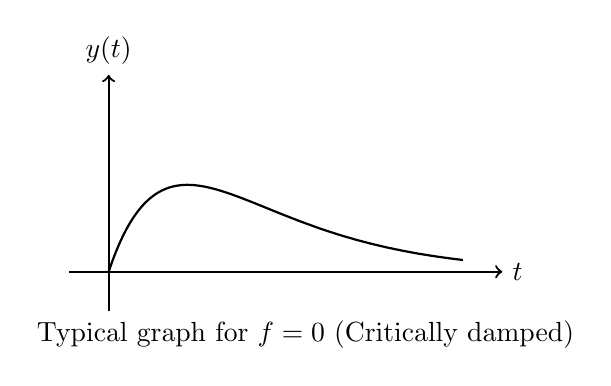
\begin{tikzpicture}[scale=1]
    \draw[->, thick] (-0.5, 0) -- (5, 0) node[right] {$t$};
    \draw[->, thick] (0, -0.5) -- (0, 2.5) node[above] {$y(t)$};
    \draw[domain=0:4.5, samples=100, thick] plot (\x, {3*\x*exp(-\x)});
    \node at (2.5, -0.8) {Typical graph for $f=0$ (Critically damped)};
\end{tikzpicture}
\end{center}

\subsubsection{Case II: $\omega^2 > a^2$ (Under-Damped)}

We start from the fundamental identities (derived via Euler's formula):
\[
\Lap[\cos(\beta t)](z) = \frac{z}{z^2 + \beta^2}, \qquad \Lap[\sin(\beta t)](z) = \frac{\beta}{z^2 + \beta^2}
\]
Let $\beta = \sqrt{\omega^2 - a^2} > 0$. Using the frequency shift property:
\[
\frac{1}{(z+a)^2 + \beta^2} = \frac{1}{\beta} \cdot \frac{\beta}{(z+a)^2 + \beta^2} = \frac{1}{\beta} \cdot \Lap[e^{-at} \sin(\beta t)](z)
\]
\[
\frac{z+a}{(z+a)^2 + \beta^2} = \Lap[e^{-at} \cos(\beta t)](z)
\]
Therefore, $Y(z)$ becomes:
\begin{align*}
Y(z) &= \Lap\left[\frac{1}{\sqrt{\omega^2 - a^2}}e^{-at}\sin(\sqrt{\omega^2 - a^2}t)\right](z) \cdot F(z) \\
&\quad + \Lap\left[e^{-at}\cos(\sqrt{\omega^2 - a^2}t)\right](z) \cdot y_0 \\
&\quad + \Lap\left[\frac{1}{\sqrt{\omega^2 - a^2}}e^{-at}\sin(\sqrt{\omega^2 - a^2}t)\right](z) \cdot (ay_0 + v_0)
\end{align*}
Taking the inverse:
\begin{align*}
y(t) &= \int_{0}^{t} \frac{1}{\sqrt{\omega^2-a^2}} e^{-a(t-s)} \sin\left(\sqrt{\omega^2-a^2}(t-s)\right)f(s)\dd s \\
&\quad + e^{-at}\cos\left(\sqrt{\omega^2-a^2}t\right)y_0 \\
&\quad + \frac{1}{\sqrt{\omega^2-a^2}}e^{-at}\sin\left(\sqrt{\omega^2-a^2}t\right)(ay_0 + v_0)
\end{align*}

\begin{center}
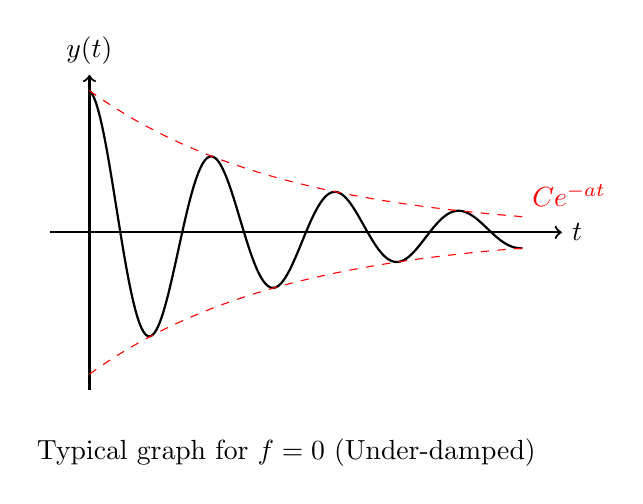
\begin{tikzpicture}[scale=1]
    \draw[->, thick] (-0.5, 0) -- (6, 0) node[right] {$t$};
    \draw[->, thick] (0, -2) -- (0, 2) node[above] {$y(t)$};
    \draw[domain=0:5.5, samples=200, thick] plot (\x, {1.8*exp(-0.4*\x)*cos(4*\x r)});
    \draw[domain=0:5.5, samples=50, dashed, red] plot (\x, {1.8*exp(-0.4*\x)}) node[above right] {$Ce^{-at}$};
    \draw[domain=0:5.5, samples=50, dashed, red] plot (\x, {-1.8*exp(-0.4*\x)});
    \node at (2.5, -2.8) {Typical graph for $f=0$ (Under-damped)};
\end{tikzpicture}
\end{center}


\subsubsection{Case III: $\omega^2 < a^2$ (Over-Damped)}

We use the hyperbolic functions:
\[
\Lap[\cosh(\beta t)](z) = \frac{z}{z^2 - \beta^2}, \qquad \Lap[\sinh(\beta t)](z) = \frac{\beta}{z^2 - \beta^2}
\]
(These can be derived using $cosh(x) = \cos(ix)$ and $\sinh(x) = -i\sin(ix)$). Letting $\beta = \sqrt{a^2 - \omega^2} > 0$:
\[
\frac{1}{(z+a)^2 - \beta^2} = \frac{1}{\beta} \Lap[\sinh(\beta t)e^{-at}](z)
\]
\[
\frac{z+a}{(z+a)^2 - \beta^2} = \Lap[\cosh(\beta t)e^{-at}](z)
\]
Following the exact same structure as Case II:
\begin{align*}
y(t) &= \int_{0}^{t} \frac{1}{\sqrt{a^2-\omega^2}} e^{-a(t-s)} \sinh\left(\sqrt{a^2-\omega^2}(t-s)\right)f(s)\dd s \\
&\quad + e^{-at}\cosh\left(\sqrt{a^2-\omega^2}t\right)y_0 \\
&\quad + \frac{1}{\sqrt{a^2-\omega^2}}e^{-at}\sinh\left(\sqrt{a^2-\omega^2}t\right)(ay_0 + v_0)
\end{align*}
The graph behavior for $f=0$ is similar to the critically damped case (a potential single peak, followed by pure exponential decay without oscillation).


\subsection{Physical Motivation and Resonance}
From Hooke's law:
\[
m \cdot y'' = f_{\text{ext}} - k \cdot y - d \cdot y' \implies y'' + \frac{d}{m}y' + \frac{k}{m}y = \frac{f_{\text{ext}}}{m}
\]
Comparing coefficients gives $\omega^2 = \frac{k}{m}$ and $2a = \frac{d}{m}$. 

\textbf{Resonance:} In the case when $a=0$ (no damping), and with $y_0 = 0, v_0 = 0$:
\[
y(t) = \int_{0}^{t} \frac{1}{|\omega|} \sin(|\omega|(t-s)) \cdot f(s)\dd s
\]
If the external forcing $f(s)$ is of the form $\sin(\gamma s)$:
\begin{itemize}
    \item If $\gamma \neq \pm \omega$: $y(t)$ remains bounded as $t \to +\infty$ ("cancellations" occur inside the integral).
    \item If $\gamma = \pm \omega$: $|y(t)| \to +\infty$ as $t \to +\infty$. The forcing frequency exactly matches the eigen-frequency of the system, causing unbounded amplitude growth.
\end{itemize}

\newpage

\subsection{The Inverse Laplace Transform}

Recall: If $\gamma_0$ is an abscissa of convergence for $f$ (meaning, in practice, that asymptotically as $t \to \infty$, $f$ behaves like $e^{\gamma_0 t}$ up to polynomial corrections), then $\Lap[f](z)$ is holomorphic (and thus has no singularities) on $\{z : \Re(z) > \gamma_0\}$.

In some sense, the "opposite" is also true: If $F(z)$ is holomorphic in $\{z : \Re(z) > \gamma_0\}$ and doesn't "grow" as $|z| \to \infty$, then $\gamma_0$ is an abscissa of convergence for some function $f$.

\begin{theorem}[Mellin Inversion Formula]
Suppose that $f: [0, +\infty) \to \C$ is a piecewise continuous function and, for some $\gamma \in \R$, $F(z) = \Lap[f](z)$ is holomorphic on the region $\{z : \Re(z) \ge \gamma\}$, and
\[
\lim_{T \to +\infty} \int_{-T}^{T} F(\gamma + i\zeta) e^{(\gamma + i\zeta)t} \dd \zeta \quad \text{exists for all } t \ge 0.
\]
(Both conditions are automatically true if some $\gamma_0 < \gamma$ is an abscissa of convergence for $f$).

\begin{center}
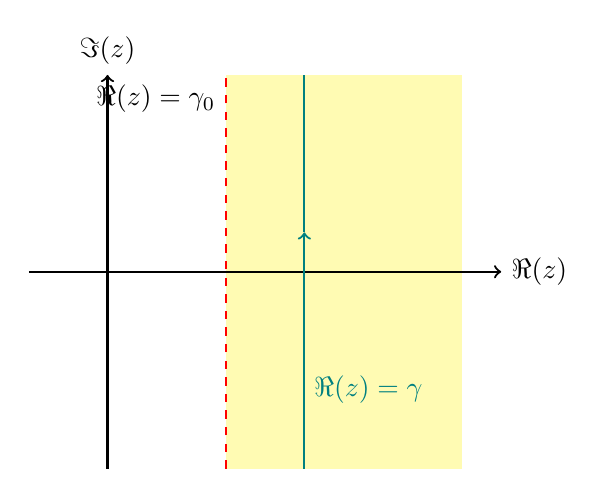
\begin{tikzpicture}[scale=1]
    \fill[yellow!30] (1.5, -2.5) rectangle (4.5, 2.5);
    \draw[->, thick] (-1, 0) -- (5, 0) node[right] {$\Re(z)$};
    \draw[->, thick] (0, -2.5) -- (0, 2.5) node[above] {$\Im(z)$};
    
    \draw[dashed, red, thick] (1.5, -2.5) -- (1.5, 2.5) node[below left, text=black] {$\Re(z)=\gamma_0$};
    
    \draw[thick, teal, ->] (2.5, -2.5) -- (2.5, 0.5);
    \draw[thick, teal] (2.5, 0.5) -- (2.5, 2.5);
    \node[teal, right] at (2.5, -1.5) {$\Re(z)=\gamma$};
\end{tikzpicture}
\end{center}

Then, $f(t)$ is uniquely determined by the Bromwich integral:
\[
f(t) = \frac{1}{2\pi} \int_{-\infty}^{+\infty} F(\gamma + i\zeta) e^{(\gamma + i\zeta)t} \dd\zeta = \frac{1}{2\pi i} \int_{\gamma - i\infty}^{\gamma + i\infty} F(z) e^{zt} \dd z
\]
\end{theorem}

\begin{verification}[Absolute vs. Principal Value Convergence]
Note: The above integral might not converge absolutely (e.g., if $f(t) = 1$ for $t \ge 0$, then $F(z) = \frac{1}{z}$ and $\int \frac{1}{|\gamma+i\zeta|} d\zeta = \infty$). So the integral is evaluated as a Cauchy Principal Value:
\[
\frac{1}{2\pi} \lim_{T \to +\infty} \int_{-T}^{+T} F(\gamma + i\zeta) e^{(\gamma + i\zeta)t} \dd\zeta
\]
\end{verification}

\begin{proofbox}
Extend $f: [0, +\infty) \to \C$ to a function on $(-\infty, +\infty)$ by setting $f(t) = 0$ for $t < 0$. 

Let $g(t) = f(t) e^{-\gamma t}$. Take the Fourier transform of $g$:
\begin{align*}
\hat{g}(\alpha) &= \frac{1}{\sqrt{2\pi}} \int_{-\infty}^{+\infty} g(t) e^{-i\alpha t} \dd t \\
&= \frac{1}{\sqrt{2\pi}} \int_{-\infty}^{+\infty} f(t) e^{-(\gamma + i\alpha)t} \dd t \\
\text{(since $f(t)=0$ for $t<0$)} \quad &= \frac{1}{\sqrt{2\pi}} \int_{0}^{+\infty} f(t) e^{-(\gamma + i\alpha)t} \dd t \\
&= \frac{1}{\sqrt{2\pi}} F(\gamma + i\alpha) \quad \text{(Laplace transform evaluated at $z = \gamma + i\alpha$)}
\end{align*}
By the inverse Fourier transform formula:
\[
g(t) = \frac{1}{\sqrt{2\pi}} \int_{-\infty}^{+\infty} \hat{g}(\alpha) e^{i\alpha t} \dd\alpha = \frac{1}{2\pi} \int_{-\infty}^{+\infty} F(\gamma + i\alpha) e^{i\alpha t} \dd\alpha
\]
Since $f(t) = g(t) e^{\gamma t}$, multiplying both sides by $e^{\gamma t}$ yields:
\[
f(t) = \frac{1}{2\pi} \int_{-\infty}^{+\infty} F(\gamma + i\alpha) e^{(\gamma + i\alpha)t} \dd\alpha
\]
\end{proofbox}

\begin{remark}[Lerch's Theorem]
\begin{enumerate}
    \item $f(t)$ is uniquely determined by $\Lap[f](z)$ through this formula (Lerch's theorem). Two functions having the same Laplace transform are identical almost everywhere.
    \item The condition on the existence of $\lim_{T \to +\infty} \int_{-T}^{T} F(\gamma+i\zeta) e^{(\gamma+i\zeta)t}\dd\zeta$ is automatically fulfilled if the absolute integrability condition $\int_{-\infty}^{+\infty} |F(\gamma+i\zeta)| \dd\zeta < +\infty$ holds.
\end{enumerate}
\end{remark}